\documentclass{beamer}
\usepackage{beamerthemeshadow}
\usepackage{mathtools}
\usepackage{fontspec}
\newcommand{\datapath} {}
%\newcommand{\referenceGenome} {reference.fasta}
%\newcommand{\reads} {reads.fastq}

%Reference genome indexing
\newcommand{\refindex}[1]{\texttt{tmap index -f #1}}

%map reads
\newcommand{\tmap}[3]{\texttt{tmap map3 -f #1 \textbackslash \\
    -r #2 \textbackslash \\
    -i fastq \textbackslash \\
    -o 2 \textbackslash \\
    -s #3
  }
}

\newcommand{\sortbam}[2]{\texttt{samtools sort #1 \textbackslash \\ #2}}

\newcommand{\reheader}[2]{\texttt{samtools view -H #1 \textbackslash \\
    | sed 's/SM:NOSM/SM:Sample1/' \textbackslash \\
    | samtools reheader - mapped\_reads.bam \textbackslash \\
    > #2
  }
}

\newcommand{\samtoolssnp}[3]{\texttt{samtools mpileup -uf #1 \textbackslash \\
    #2 \textbackslash \\
    | bcftools call -cv \textbackslash \\
    | vcfutils.pl varFilter > #3
  }
}


\begin{document}
\begin{frame}{SNP calling}
  \frametitle{Pipeline overview}
  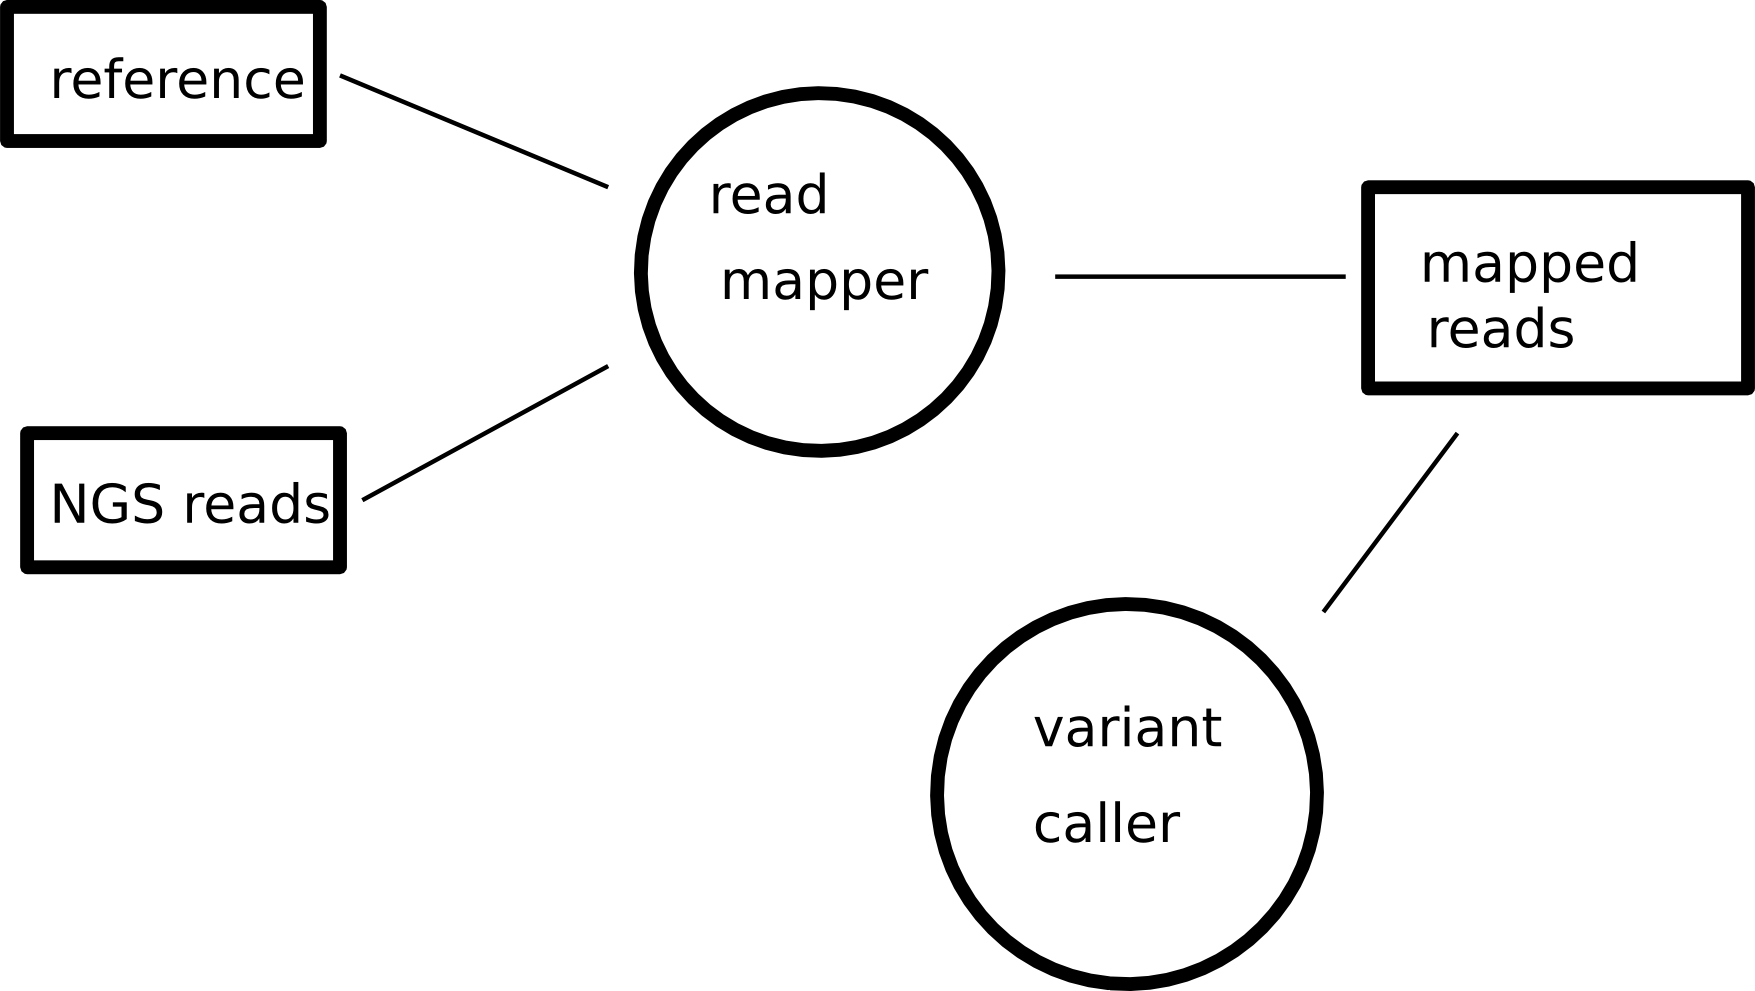
\includegraphics[width=\linewidth, keepaspectratio]{pic/pipe_overview.png}
\end{frame}

%Prepare reference genome and map reads
\begin{frame}{Read mapping}
  \begin{itemize}
    \item Index reference genome (need to do it only once per reference)
  \end{itemize}
  \refindex{reference.fasta}
  \pause
  \begin{itemize}
    \item Map reads against reference genome
  \end{itemize}
  \tmap{reference.fasta}{reads.fastq}{mapped\_reads.bam}
\end{frame}

%BAM file specification
\begin{frame}{BAM file}
  \begin{itemize}
    \item Let's see what is inside the bam file
  \end{itemize}
  \texttt{samtools view mapped\_reads.bam | head -n 20}
\end{frame}

{
\usebackgroundtemplate{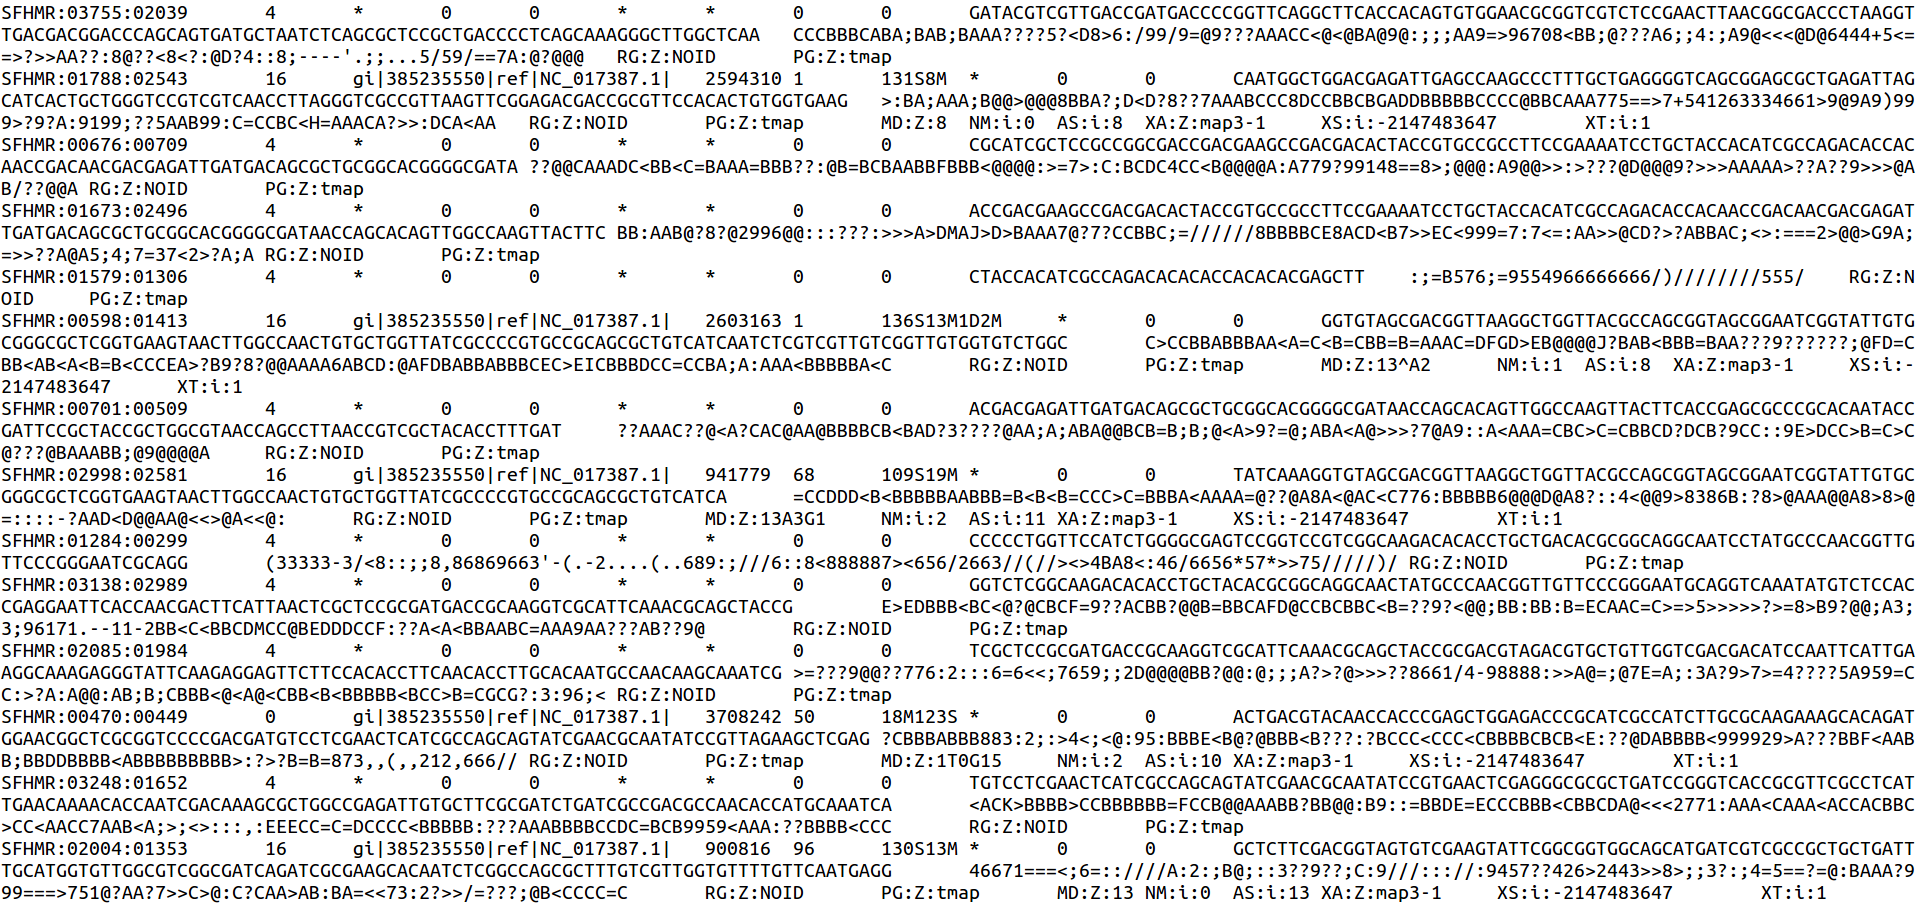
\includegraphics[width=\paperwidth, height=\paperheight]{pic/bam.png}}
\begin{frame}[plain]
\end{frame}
}

%More info: http://samtools.github.io/hts-specs/SAMv1.pdf
\begin{frame}{BAM file format}
  \framesubtitle{The header}
    \begin{itemize}
      \item Let's look at the bam header
     \end{itemize}
  \texttt{samtools view -H mapped\_reads.bam} \\~\\
  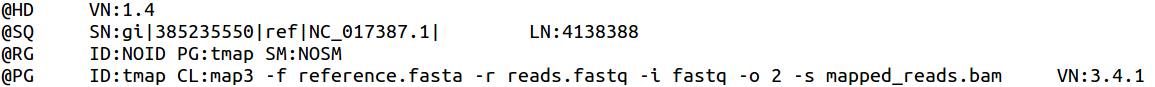
\includegraphics[width=\linewidth, keepaspectratio]{pic/bam_head.png}
\end{frame}

%Lets change the header so it includes our sequencing platform and sample name
\begin{frame}{BAM file header modifying}
  \begin{itemize}
    \item Let's change the header so that it includes our sample name!
  \end{itemize}
  \reheader{mapped\_reads.bam}{mapped\_reads.reheaded.bam}
\end{frame}

%Lets change header give the mapper our sample name and sequencing platform


%Call variants
\begin{frame} {Variant calling}
  \begin{itemize}
    \item Variant callers need sorted bam file
  \end{itemize}
  \sortbam{mapped\_reads.reheaded.bam}{mapped\_reads.reheaded.sorted}
\end{frame}

\begin{frame}{Variant calling}
  \samtoolssnp{reference.fasta}{mapped\_reads.reheaded.sorted.bam}{variants.samtools.vcf}
\end{frame}

%VCF file format
\begin{frame}{Variant call format (VCF)}
  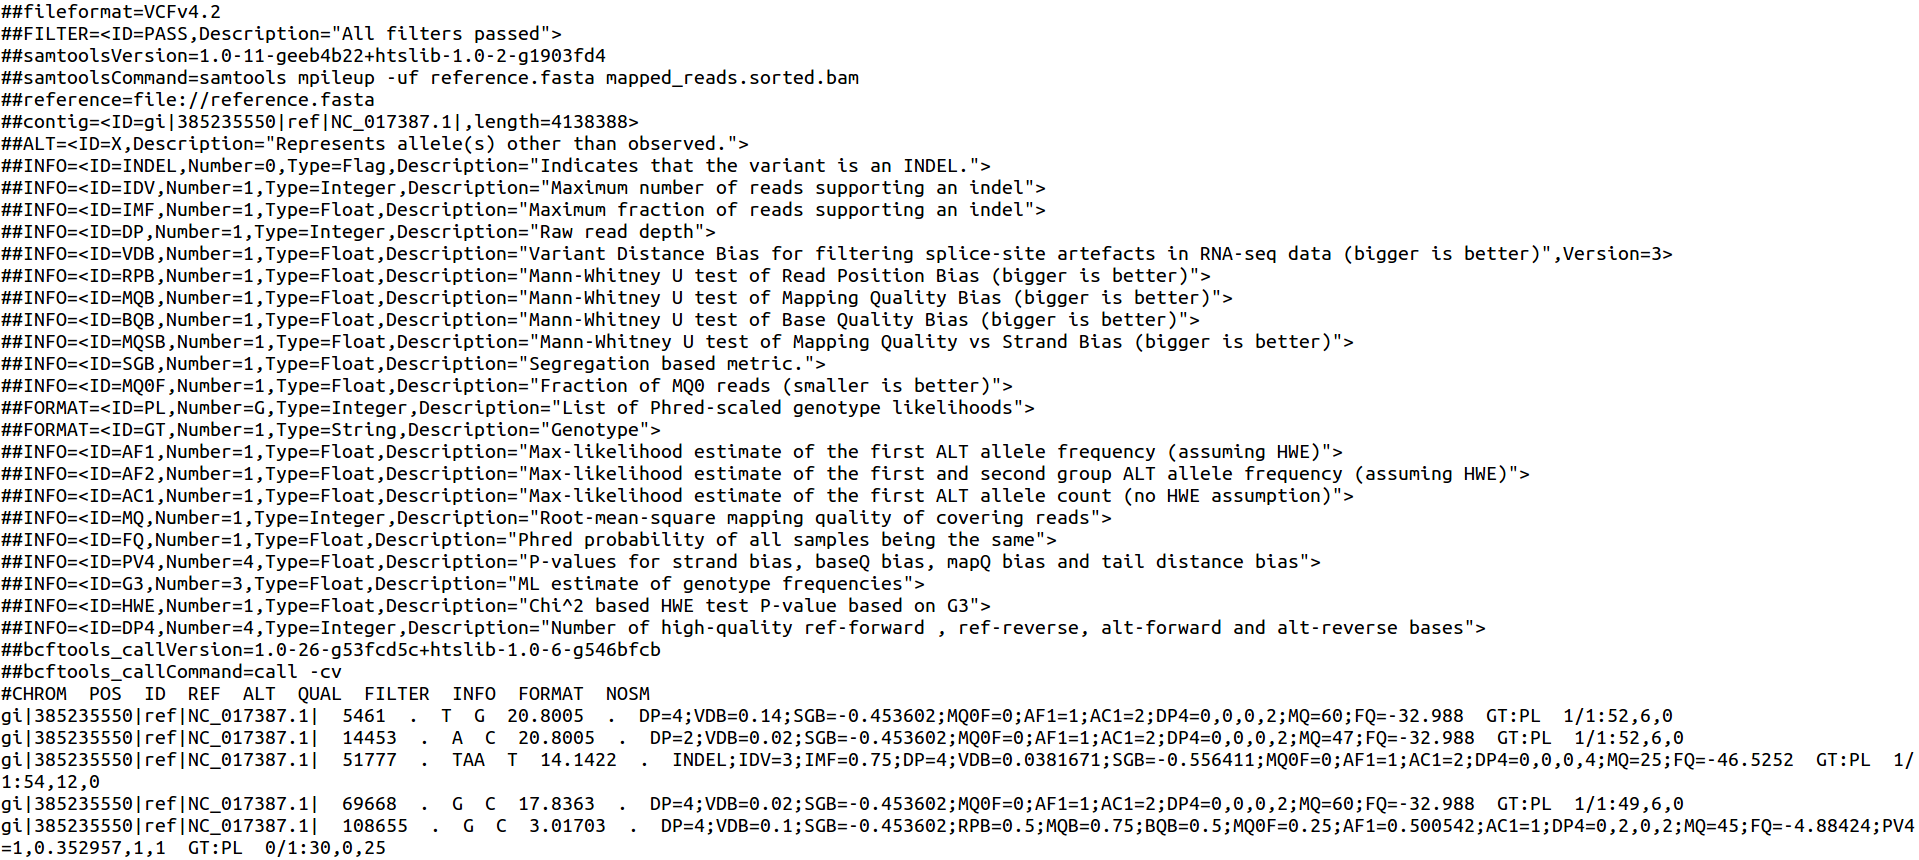
\includegraphics[width=\paperwidth, keepaspectratio]{pic/vcf.png}
\end{frame}

%Pipeline building

%command line summary
\begin{frame}{Summary of used commands}
  
  \begin{itemize}
    \item Reference genome indexing
  \end{itemize}
  \refindex{reference.fasta}\\~\\

  \begin{itemize}
    \item Read mapping against reference genome
  \end{itemize}
  \tmap{reference.fasta}{reads.fastq}{mapped\_reads.bam}\\~\\
  
  \begin{itemize}
    \item Bam header modifying
  \end{itemize}
  \reheader{mapped\_reads.bam}{mapped\_reads.reheaded.bam}
\end{frame}

\begin{frame}

  \begin{itemize}
    \item Mapped read sorting
  \end{itemize}
  \sortbam{mapped\_reads.reheaded.bam}{mapped\_reads.reheaded.sorted}

  \begin{itemize}
    \item Variant calling
  \end{itemize}
  \samtoolssnp{reference.fasta}{mapped\_reads.reheaded.sorted.bam}{variants.samtools.vcf}
\end{frame}

%Pipeline building
\begin{frame}
  \frametitle{Let's build pipeline!}
  \tmap{reference.fasta}{reads.fastq}{mapped\_reads.bam}\\~\\
  \reheader{mapped\_reads.bam}{mapped\_reads.reheaded.bam}\\~\\
  
  \sortbam{mapped\_reads.reheaded.bam}{mapped\_reads.reheaded.sorted}\\
  \samtoolssnp{reference.fasta}{mapped\_reads.reheaded.sorted.bam}{variants.samtools.vcf}
\end{frame}

%GATK pipeline uz hromosomas fragmentu
%Lets change header so it includes our sample name
\end{document}
